\section{Design of the track}

In order to validate that the requirements of the project are met. A track for the bus which is designed based on the requirements had to be made. This section will detail the design decisions made when designing this track. 

%Firstly the setup
First, let us start with a short reminder: The track should have two lanes, as to mimic the pre-existing infrastructure, which usually has bidirectional roads. Furthermore, the track should have bus stops that the vehicle can drive into, such that passengers can get on/off the bus. The bus stops need to have a minimum length equivalent to the length of the bus in addition to the space that is needed to drive into and out of the bus stops.

Based on this the we know that the track should have proportions based on the scale of the bus. Also we know that the track should include turns as sharp as in real life\cite{DriveingCurves}. The width of the road should also be designed after real danish roads based on the laws given by the Danish road directorate \cite{roadRules}.  As such the track needs to be designed such that the bus has the needed space to turn smoothly.

To help the sensors detect when to switch to a bus stop lane, the track should have special coloured tape placed a specified distance away from the bus stops, which sensor(s) can recognise.

To draw the track that the bus will drive on, black tape is used such that the sensors, which perform line tracking can detect the lines. The sensors are more effective at detection when working with colours with strong contrast, therefore we chose black and white. Black tape and white backdrop have been chosen over white tape and black backdrop. White lines and black backdrop are more true to life, but the results are the same, so since a white backdrop was more accessible, this was chosen.

Bus stops can in principle come in many forms, however, we will focus on a single bus stop design. This design must have enough space

The following is a brief explanation of the relevant rules that real life roads must follow and therefore our track has to follow. There are of course allot of rules, that are irrelevant for this project, e.g. the thickness of a road. 

%Calculated based on the danish road directorate, see "Calculation of maximal turn angle of a bus road" in appendix \ref{laneCalculations}, if a 12 meter bus can drive on a road with with a front wheel turn angle of 28.6 with a 0.3 meter leeway to each side at 15 km/t\cite{DriveingCurves}. this is the simple turn where the bus has no room to perform a small turn to the opposite direction to make a sharper turn, see\cite{DriveingCurves} for a illustration of the manoeuvre.

The minimal width of the road, set forth by the road directorate, is not constant. On a straight or mildly curving road, the standard width of the road is 3.5 meters. However, when the road has a sharp turn the road other rules apply. 

Let us start with the rules for straight roads as previously stated a bus road in the city has to be 3.5 meters wide\cite{roadRules}. 3 meters is allowed on short straight stretches, however, this is not the standard so this number is discarded for now. We also know from the Danish road directorate that the maximum width of the bus is 2.55 meters\cite{DriveingCurves}. From this the proportions are calculated, see 1 in appendix \ref{laneCalculations} for the specific calculations.

For the curved roads, the Danish road directorate has set forth a number of conditions for the approval of roads and the vehicles that are allowed to use the road. In order for a bus of 12 meters in length to be allowed to drive on a road, the road has to abide by the following condition.
A bus 12 meters in length, must be able to pass through the road with a front wheel turning angle of maximum  28.6 degrees, see 2.1 in appendix \ref{laneCalculations}, while keeping 0.3 meters leeway to each side at any point\cite{DriveingCurves}, or it must have an area to be able to turn a bit to the opposing side, so that it can make a sharper turn. However, we have chosen to refer to the simple turn as our requirement. According to these requirements, the calculations found in section 2 appendix \ref{laneCalculations} were made, to ensure that the track conforms to this rule.
The length of the bus stop has been found by finding the minimum distance that the bus needs to drive into and out of the bus lane, and then added to the length of the bus. The formula can be seen in \cite{busstoplength} and comes out to ~56.4. However, this would require the bus to enter the bus stop at a very steep angle that will not be possible at most roads, so a big amount of additional space has been added to the bus stop.

According to these rules, the following design in Figure \ref{fig:TrackDesign} was made. The image is not to scale.

\begin{figure}[ht]
    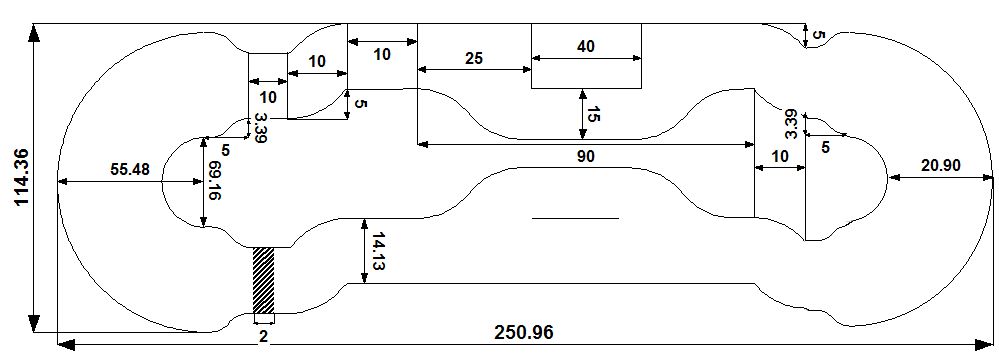
\includegraphics[width=1\textwidth]{Images/Design/TrackDesign.PNG}
    \caption{Track design}
    \label{fig:TrackDesign}
\end{figure}






%Straight bus lane calculations -1
%Calculation of maximal turn angle of a bus road -2.1
%From straight to turning width calculations -3
%Turning bus lane radius calculation -2


%beskriv bus stop: 45 grader ind, 45 grader ud, bus bredde + 2 cm, bus længde 
%der er mange forskellige busstoppesteder, så vi vælger bare et design